\section{Cloud Architektur}

Innerhalb von Cloud Architekturen gibt es drei verschiedene Rollen:
\begin{itemize}
	\item \textbf{Provider:} bietet Cloud Produkte/Lösungen an
	\item \textbf{Konsumenten:} konsumieren Cloudlösungen
	\item \textbf{Klienten:} nehmen Cloudlösungen (Anwendungen/Daten) in Anspruch
\end{itemize}

\subsection{Konzeptuelle Sichtweise}

In diesem Abschnitt werden die Architekturen der einzelnen Kategorien von Cloudlösungen beschrieben.

\subsubsection{Konsumenten Sichtweise}
Ressourcen werden in Form von Clustersystemen vom Provider zur Verfügung gestellt(siehe \textbf{Abbildung \ref{ConsumerView}}).
Einzelne Klienten können über eine Netzwerkverbindung auf diese Ressourcen zeitgleich zugreifen. Der Provider kann außerdem den Pool
von Hardware Ressourcen verwalten, d.h. einzelne Hardware kann stillgelegt und ersetzt werden. Die Klienten werden nach dem Stilllegen
auf andere Hardware Ressourcen weitergeleitet.
\begin{figure}[h]
    \centering
	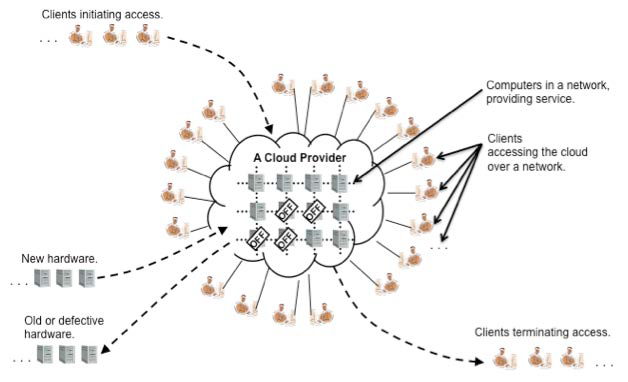
\includegraphics[width=0.5\textwidth]{Images/ConsumerView}
	\caption{Konsumenten Sichtweise \cite{Badger}}
	\label{ConsumerView}
\end{figure}
Alle Kategorien von Cloud-Computing können sogenannte Sicherheitsperimeter verwenden. Diese regeln den Zugriff auf die Ressource \cite{Badger}.

\subsubsection{Lokale Private Cloud}
Klienten, die sich innerhalb des Sicherheitsperimeters befinden, können sich mit der privaten Cloud verbinden (siehe \textbf{Abbildung \ref{PrivateCloud}}). 
Klienten von außerhalb, können eine Verbindung durch den \glqq boundary controller\grqq{} aufbauen. Die Cloud und die Sicherheitsperimeter werden von dem Konsumenten verwaltet.
\begin{figure}[h]
    \centering
	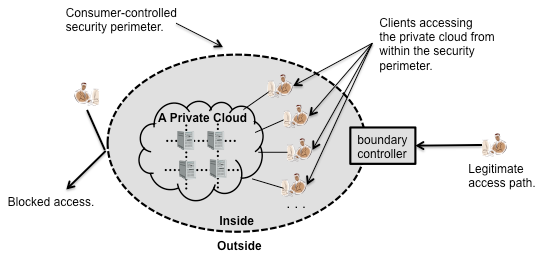
\includegraphics[width=0.5\textwidth]{Images/On-sitePrivateCloud}
	\caption{Private Cloud \cite{Badger}}
	\label{PrivateCloud}
\end{figure}
Dieser muss die Cloud so einstellen, dass die Arbeitslast zwischen verschiedenen Maschinen verteilt werden kann, um die Ressourcen optimal nutzen zu können. Außerdem sollten redundante Kopien der Daten auf verschiedenen Maschinen 
gespeichert werden. Dies hat den Vorteil, dass bei einem Serverausfall der Klient auf eine andere Maschine weitergeleitet werden kann.
Außerdem muss der Konsument sicherstellen, dass wichtige Daten wie z.B. Lohnabrechnungen nicht von allen Klienten zugegriffen werden können,
da verschiedenen Daten auf einer Maschine verarbeitet werden können. Der Nachteil von privaten Clouds sind die hohen Anschaffungskosten und fehlende Flexibilität der Infrastruktur bei steigenden Zugriffszahlen, da die dafür benötigte Hardware vom Konsumenten bereitgestellt werden \cite{Badger}.

\subsubsection{Ausgelagerte Private Cloud}

Bei der ausgelagerten Privaten Cloud, wird die Cloud zu einem Provider verlagert. Dieser separiert das Organisationsnetzwerk
von seinem \glqq öffentlichen\grqq{} Netzwerk, wie in \textbf{Abbildung \ref{OutSourcedPrivateCloud}} zu sehen ist. Das Netzwerk wird vom Provider
durch einen Sicherheitsperimeter geschützt. Der Provider muss dabei sicherstellen, dass die Sicherheitsanforderungen des Konsumenten erfüllt werden. 
Der Konsument kann ebenfalls einen Sicherheitsperimeter in seiner Organisation installieren, um den Zugriff zur Cloud zu regeln.
Die beiden Perimeter werden dann durch einen Kommunikationskanal verbunden und Klienten können dann nur über diesen Kanal auf Daten der Cloud zugreifen.
\begin{figure}[h]
    \centering
	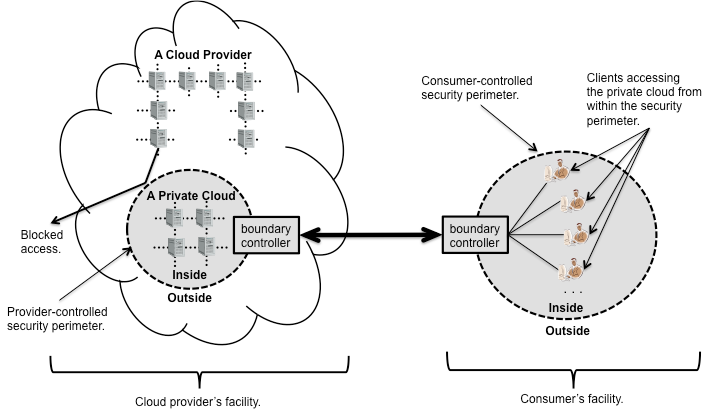
\includegraphics[width=0.5\textwidth]{Images/OutSourcedPrivateCloud}
	\caption{Ausgelagerte Private Cloud \cite{Badger}}
	\label{OutSourcedPrivateCloud}
\end{figure}
Der Konsument ist in diesem Fall von der Netzwerkverfügbarkeit und -geschwindigkeit des Providers abhängig, kann die Geschwindigkeit aber durch Sondertarife erhöhen.
Der Provider muss außerdem sicherstellen, dass die Arbeitslast auf den verschiedenen Maschinen innerhalb des Perimeters verteilt wird und sich die Daten 
nicht mit den Daten von anderen Organisationen, außerhalb des Perimeters, vermischen.
Der Vorteil dieser Architektur ist es, dass der Konsument keine eigenen Ressourcen mehr anschaffen muss und diese beim Provider mieten kann \cite{Badger}.

\subsubsection{Lokale Community Cloud}

Bei der lokalen Community Cloud teilen mehrere Organisationen ihre Ressourcen und Daten. Alle Organisationen stellen und/oder konsumieren Cloud Services.
Dabei muss mindestens eine Organisation solche Services zur Verfügung stellen, sprich Provider sein.
Sollte jede Organisation einen Sicherheitsperimeter installieren, werden die einzelnen Organisationen durch Kommunikationskanäle zwischen den \glqq boundary controller\grqq{}{}{}{} verbunden.
Organisationen können außerdem einen weiteren Sicherheitsperimeter einrichten, um die lokalen Cloud Ressourcen von den lokalen Ressourcen zu trennen.
\begin{figure}[h]
    \centering
	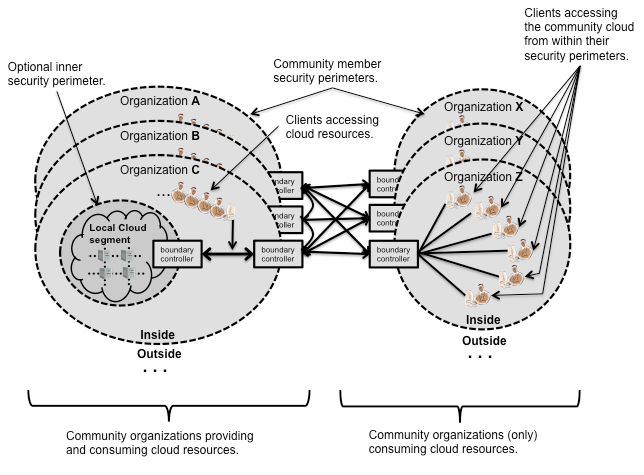
\includegraphics[width=0.5\textwidth]{Images/On-siteCommunityCloud}
	\caption{Lokale Community Cloud \cite{Badger}}
	\label{On-siteCommunityCloud}
\end{figure}
Für die Verwendung der lokalen Community Cloud wird eine komplexe Sicherheitsauthentifizierung benötigt. Jede Organisation der Community muss einen Zugriff bieten und erhalten.
Außerdem müssen die Kommunikationskanäle geschützt und bei der Verwendung des öffentlichen Internet Kryptographie verwenden werden. Die einzelnen Kommunikationskanäle zwischen den Teilnehmern 
können verschiedene Level der Performance, Sicherheit und Zuverlässigkeit bereitstellen, abhängig von den Ansprüchen der Teilnehmenden Organisationen. Die Sicherheit der einzelnen Clouds hängt 
hierbei von den den Sicherheitsperimeter der einzelnen Organisationen ab. Ein großer Nachteil dieser Methode sind die hohen Kosten der einzelnen Provider, die Ressourcen 
anschaffen und Services konfigurieren müssen. Die Konsumenten hingegen zahlen nur die Mietkosten der für die Verwendungen der einzelnen Clouds. Der Nachteil ist hier analog zur lokalen privaten Cloud \cite{Badger}.

\subsubsection{Ausgelagerte Community Cloud}

Bei der ausgelagerten Community Cloud verhält es sich ähnlich zur ausgelagerten privaten Cloud, wie in \textbf{Abbildung \ref{OutSourcedCommunityCloud}} zu sehen ist.
Um die serverseitige Verantwortung kümmert sich hier der Provider, der einen Sicherheitsperimeter installiert und verwaltet. Dabei sorgt der Provider dafür, dass sich 
die Community Ressourcen und die Cloud Provider Ressourcen, die sich außerhalb des Perimeters befinden, nicht vermischen. Ein wesentlicher Unterschied zur ausgelagerten privaten Cloud
besteht darin, dass der Cloud Provider möglicherweise eine Freigaberichtlinie zwischen den teilnehmenden Unternehmen der Community Cloud durchsetzen muss. 
Um den Konsumenten eine Verbindung zur Cloud zu ermöglichen, müssen sichere Kommunikationskanäle zwischen den einzelnen Organisationen und 
dem Provider installiert werden \cite{Badger}.

\begin{figure}[h]
    \centering
	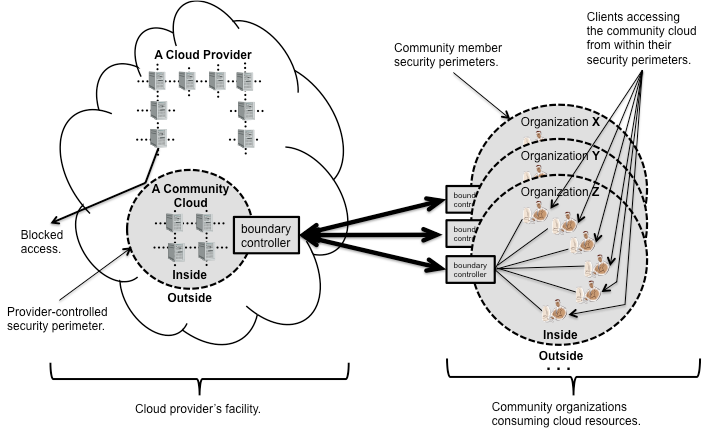
\includegraphics[width=0.5\textwidth]{Images/OutSourcedCommunityCloud}
	\caption{Ausgelagerte Community Cloud \cite{Badger}}
	\label{OutSourcedCommunityCloud}
\end{figure}

\subsubsection{Public Cloud}

Die Public Cloud, die in \textbf{Abbildung \ref{PublicCloud}} zu sehen ist, verhält sich recht ähnlich zu \textbf{Abbildung \ref{ConsumerView}}.
Außer das der Konsument einen eigenen Sicherheitsperimeter installiert, um den Zugriff zur Cloud zu regeln.

 
\begin{figure}[h]
    \centering
	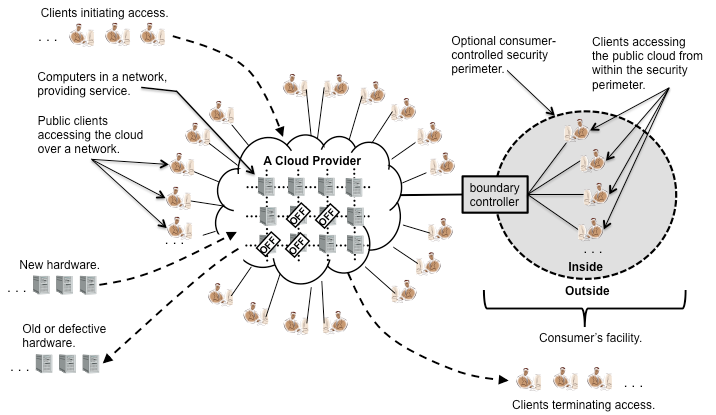
\includegraphics[width=0.5\textwidth]{Images/PublicCloud}
	\caption{Public Cloud \cite{Badger}}
	\label{PublicCloud}
\end{figure}

In diesem Szenario verbindet sich der Konsument über das öffentliche Internet, sodass die Verbindungsqualität und -zuverlässigkeit zur Cloud
von dem Internet Provider, dem DNS Server und der Router Infrastruktur abhängt. Die Arbeitslast oder Ressourcen eines Konsumenten können zu jeder Zeit
vom Provider migriert werden. Ein großer Vorteil der Public Cloud ist die Kosteneffizienz, da Datenzentren an Standorten verwendet werden können, die für den Konsumenten am günstigen sind.
Ein Beispiel dafür wäre, dass die Arbeitslast eines deutschen Unternehmens in einem deutschem Datenzentrum verarbeitet und somit die Performance verbessert wird (kurze Übertragungswege).
Dies wird aber meist nicht von Provider versichert. Die Arbeitslast kann an verschiedenen Standorten (Europa, USA, China usw.) verarbeitet werden, außer der Provider bietet eine
Standortbeschränkung an. Ein großes Problem der Public Cloud ist es, dass eine Maschine die Daten von mehreren Konsumenten verarbeiten kann und somit ein Sicherheitsrisiko entstehen kann.
Außerdem haben die Konsumenten keine Möglichkeit die Einsicht ihrer Daten zu überwachen oder eine Authentifizierung für ihre Daten einzurichten. Da große Anbieter meist eine Monitoring für die
Daten durchführen, um die tatsächliche Datennutzung zu ermitteln und den Konsumenten diese dann in Rechnung zu stellen, ist diese Methode nicht für sensible oder wichtige Daten geeignet.
Außerdem kann der Konsument nie sicher sein, ob seine Daten auch gelöscht werden, wenn er den Vertrag kündigt. 
Ein großer Vorteil der Public Cloud ist die Uneingeschränktheit in Hinsicht des Standortes und der Größe. D.h. die Größe der zur Verfügung gestellten Ressourcen lässt sich 
meist \glqq uneingeschränkt\grqq{} erhöhen oder vermindern \cite{Badger}.
Bekannte Public Cloud Provider sind Amazon Web Services (AWS) und Microsoft Azure. 
% \subsubsection{Hybrid Cloud}
% Eine Hybrid Cloud besteht aus mindestens zwei oder mehreren Privaten, Community oder Public Clouds.
% \begin{figure}[H]
%     \centering
% 	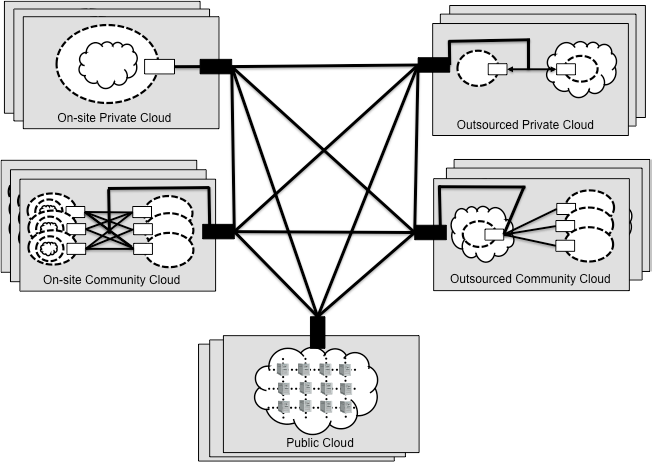
\includegraphics[width=0.5\textwidth]{Images/HybridCloud}
% 	\caption{Hybrid Cloud \cite{Badger}}
% 	\label{HybridCloud}
% \end{figure}

\subsection{Architekturen der Dienstmodelle}
In diesem Abschnitt werden die Architekturen der Dienstmodelle beschrieben.

\subsubsection{SaaS}\label{SaaS Architektur}
\begin{figure}[h]
    \centering
	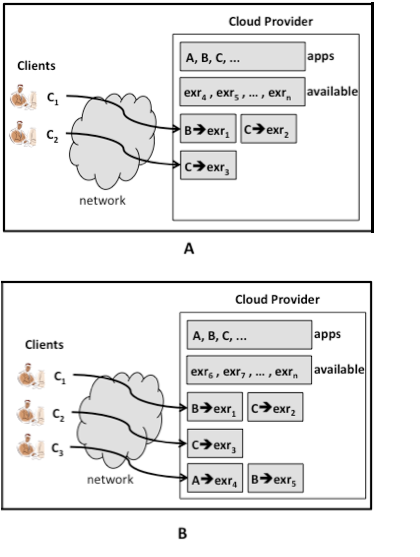
\includegraphics[width=0.5\textwidth]{Images/SaaSInteraction}
	\caption{SaaS Interaktion \cite{Badger}}
	\label{SaaSInteraction}
\end{figure}
Wie bereits in Abschnitt \ref{IaaS} beschrieben, stellt der Provider den Klienten Anwendungen (\glqq Apps\grqq{}{}) zu Verfügung.
Diese Anwendungen können dann über das öffentliche Internet (Webseiten) aufgerufen werden.
Wie in \textbf{Abbildung \ref{SaaSInteraction}} zu sehen ist, kann ein Provider mehrere Apps anbieten und ausführen.
Er hat dabei eine gewisse Anzahl an \glqq Execution Ressources\grqq{}{} (exr) zur Verfügung. 
Dabei wird den Klienten bei jedem Starten einer Anwendung eine exr zugewiesen. Sollten neue Klienten hinzukommen, werden ihnen verbleibende Ressourcen (exr) zugewiesen. 

\begin{figure}[h]
    \centering
	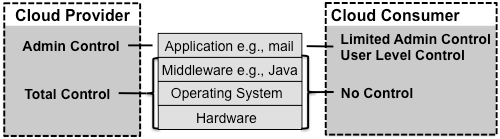
\includegraphics[width=0.5\textwidth]{Images/SaaSControl}
	\caption{SaaS Kontrollverteilung \cite{Badger}}
	\label{SaaSControl}
\end{figure}
\textbf{Abbildung \ref{SaaSControl}} zeigt, wie die Kontroll- und Managementverantwortung zwischen dem Provider und den Konsumenten verteilt wird.
Bei Software as a Service hat der Konsument nur die Kontrolle auf der Benutzerebene, d.h. dieser kann Benutzerverwalten wie z.B. Benutzer hinzufügen.
Der Provider hingegen verfügt die totale Kontrolle über alle Bereiche. Dieser ist verantwortlich für das erstellen, konfigurieren und verwalten der Anwendungen, 
sodass der Konsument diesen Service nutzen kann.
Der Provider kontrolliert die Hardware, das Betriebssystem und die Middleware \cite{Badger}.

\subsubsection*{Vorteile von SaaS}

Im Vergleich zu traditionellen Computing- und Softwareverteilungslösungen bieten SaaS-Clouds Skalierbarkeit und verlagern zudem die Belastungen vom Konsumenten zum Provider.
Die Vorteile solcher Services sind, dass für öffentliche und ausgelagerten Szenarien, sich der Großteil der von einer Anwendung verwalteten Daten auf den Softwareverteilungslösungen
des Cloud-Providers befinden. Der Provider kann diese Daten dezentral und redundant speichern, sodass ein Verlust von Daten unwahrscheinlich wird. Außerdem bieten SaaS-Provider
ein professionelles Management System an, dass z.B. Compilance-Check (Datenschutz), Security-Scanning (Virenprüfung), Backup und Disaster Recovery unterstützt.

\subsubsection*{Funktionsweise von SaaS}

Wie bereits erwähnt wird bei Start einer Anwendung von einem Nutzer ein Prozess (exr) gestartet. Dabei haben die Provider meist eine statische oder eine dynamische
Lösung, um die Anwendung zu betreiben, wie \textbf{Abbildung \ref{SaaSM1}} zeigt.
\begin{figure}[h]
    \centering
	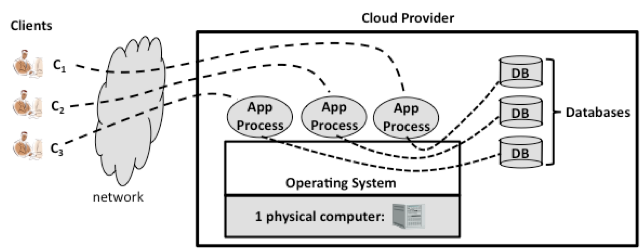
\includegraphics[width=0.5\textwidth]{Images/SaaSM1}
	\caption{Möglichkeit 1 \cite{Badger}}
	\label{SaaSM1}
\end{figure}
In diesem Szenario wird eine aktive Kopie der Anwendung für jeden Benutzer gestartet. Jede Anwendung betreibt dabei ein eigenes Datenbanksystem, indem die Daten der Benutzer gespeichert werden.
Somit besitzt jeder Klient eine eigene Kopie der Daten. Die einzelnen Kopien der Anwendung, der Datenbanksysteme und die Separierung der Benutzer wird durch das Betriebssystem ermöglicht.
Ein großer Nachteil dieses Szenarios ist es, dass hohe Kosten für das Betreiben und Synchronisieren der einzelnen Datenbanksysteme entstehen.
\begin{figure}[h]
    \centering
	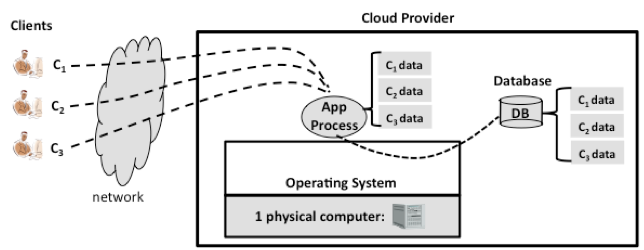
\includegraphics[width=0.5\textwidth]{Images/SaaSM2}
	\caption{Möglichkeit 2 \cite{Badger}}
	\label{SaaSM2}
\end{figure}
Beim statischen Szenario(siehe \textbf{Abbildung \ref{SaaSM2}}) wird die Anwendung vom Provider so implementiert, sodass mehrere Klienten gleichzeitig daran arbeiten können und die Daten in nur einem Datenbanksystem gespeichert werden. 
Dies hat den Vorteil das die Kosten für den Provider gesenkt werden, da nur noch eine Anwendung betrieben wird.
Die Anwendung selbst, muss dafür aber die Daten mehrerer Klienten gleichzeitig verarbeiten und trotzdem sicherstellen, dass die Sicherheit der Daten gewährleistet ist \cite{Badger}.

\subsubsection{PaaS}
Der Unterschied von PaaS zu SaaS ist, dass Konsumenten die Möglichkeit haben, eigene Anwendungen bei dem Cloud Provider betreiben zu lassen.
\begin{figure}[h]
    \centering
	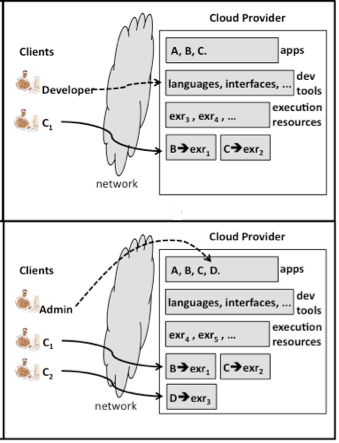
\includegraphics[width=0.5\textwidth]{Images/PaaSInteraction}
	\caption{PaaS Interaktion \cite{Badger}}
	\label{PaaSInteration}
\end{figure}
In der \textbf{Abbildung \ref{PaaSInteration}} wird gezeigt, wie sich die Interaktionen der einzelnen Nutzer verändern.
Der Klient kann weiterhin auf die Anwendungen (A, B, C) zugreifen. Beim Zugreifen wird hier ebenfalls ein neuer Prozess (exr) gestartet. Der Unterschied hier ist aber, dass
der Konsument für die Bereitstellung, Verwaltung, Aktualisierung der Anwendung zuständig ist. Der Provider bietet dem Konsumenten nur die Ressourcen um die Anwendung(en) zu betreiben.
Außerdem kann ein Provider ebenfalls Entwicklungswerkzeuge anbieten, die von den Entwicklern des Konsumenten verwendet werden können (z.B. eigene Datenbank).
\begin{figure}[h]
    \centering
	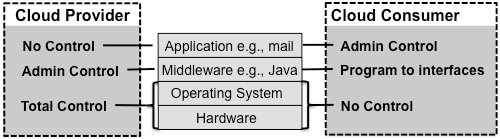
\includegraphics[width=0.5\textwidth]{Images/PaaSControl}
	\caption{PaaS Kontrollverteilung \cite{Badger}}
	\label{PaaSControl}
\end{figure}
Bei der Kontrolle der Schichten hat der Provider nur noch die Kontrolle über das Betriebssystem und die Hardware, wie die \textbf{Abbildung \ref{PaaSControl}} zeigt.
Sollte der Provider noch Entwicklungswerkzeuge anbieten, so behält er die Administrative Kontrolle über diese Werkzeuge. Der Konsument hingegen hat im Gegensatz zu SaaS,
die volle Kontrolle über die Anwendungen und falls er keine Entwicklungswerkzeuge nutzt, über die Middleware Schicht \cite{Badger}. 

\subsubsection*{Vorteile von PaaS}

PaaS teilt viele der Vorteile von SaaS, aber im Gegensatz zu SaaS hat der Konsument mehr Freiheiten und Kontrolle über die Anwendungen.
Wobei bei SaaS der Konsument und seine Klienten von der Anwendung des Providers abhängig sind. Dies verschafft den Konsumenten eine deutliche erhöhte Sicherheit über den Ablauf
der Anwendung und seiner Daten.
Der Provider kümmert sich weiterhin um ein stabiles und sicheres Netzwerk, dass eine hohe Performance von verschiedenen Standorten der Welt verspricht.
Außerdem sind auch hier die Ressourcen skalierbar, dass dem Konsumenten Flexibilität ermöglicht. 

\subsubsection{IaaS}
Bei Infrastructure as a Service erhält der Konsument eigene virtuelle Maschinen, die er verwalten und konfigurieren kann. Dabei bieten verschiedene Anbieter auch mehrere Betriebsysteme an, z.B.
Linux- oder Windowsserver. Hier muss der Konsument sich ebenfalls um die Installation und Verwaltung der einzelnen Bibliotheken, sowie die Installation einer Datenbank oder Middleware (z.B. Java) kümmern.
Somit erhöht sich der allgemeine Verwaltungsaufwand des Konsumenten. Der Provider hingegen stellt nur noch die Ressourcen und die virtuelle Maschine zur Verfügung. 
\begin{figure}[h]
    \centering
	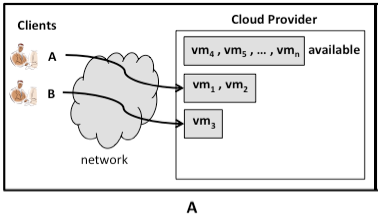
\includegraphics[width=0.5\textwidth]{Images/IaaSInteraction}
	\caption{IaaS Interaktion \cite{Badger}}
	\label{IaaSInteraction}
\end{figure}
In \textbf{Abbildung \ref{IaaSInteraction}} sieht man, dass der Provider eine bestimmte Menge (N) an virtuellen Maschinen den Konsumenten zur Verfügung stellt. Klienten können dann über ein Netzwerk, auf diese VMs zugreifen.
\begin{figure}[h]
    \centering
	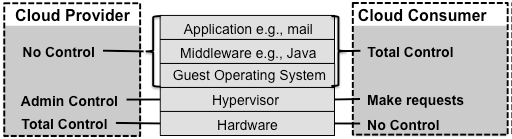
\includegraphics[width=0.5\textwidth]{Images/IaaSControl}
	\caption{IaaS Kontrollverteilung \cite{Badger}}
	\label{IaaSControl}
\end{figure}
Im Softwarestack (\textbf{Abbildung \ref{IaaSControl}}) sieht man, dass der Provider nur noch die Kontrolle auf Hardware und den Hypervisor besitzt.
%Ein Hypervisor ist ein Virtual Machine Monitor(VMM), der die Hardware verwendet, um eine oder mehrere Virtuelle Maschinen (VM) zu erstellen, dabei ist jede VM eine effiziente, isoliertes Kopie einer realen Maschine.
Im Gegensatz dazu kontrolliert der Konsument das Gast Betriebssystem, die Middleware (z.B. Java) und die Anwendung \cite{Badger}.

\subsection{Logische Sichtweise}
Eine IaaS Cloud muss Ressourcen sowohl leistungs-als auch kosteneffizient bereitstellen, wobei die Fähigkeit zur Skalierung ohne Unterbrechung des Betriebs erhalten bleiben muss.
Um die Funktionsweise eines IaaS Systems zu verstehen, gehen wir in diesem Abschnitt näher auf die einzelnen Komponenten einer Cloud ein.
\begin{figure}[h]
    \centering
	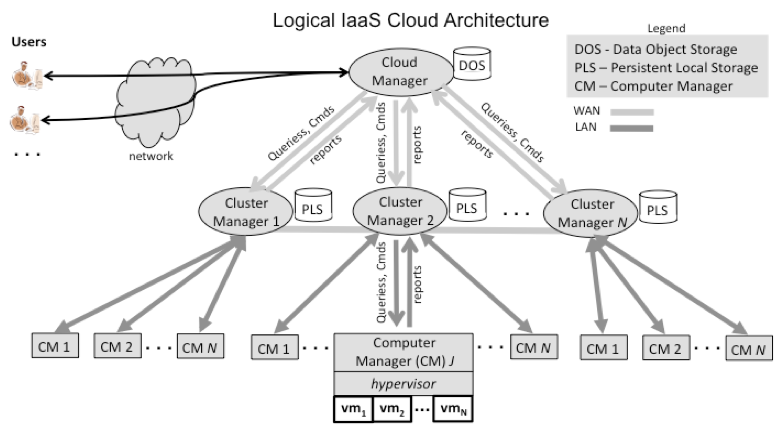
\includegraphics[width=0.5\textwidth]{Images/IaaSLogic}
	\caption{IaaS Logische Sichtweise (vgl. \cite{Badger})}
	\label{IaaSLogic}
\end{figure}
\textbf{Abbildung \ref{IaaSLogic}} zeigt, dass eine IaaS Cloud aus drei Teilen besteht:
\begin{enumerate}
	\item Cloud Manager
	\item Cluster Manager
	\item Computer Manager
\end{enumerate}

\subsubsection{Cloud Manager}
Die einzelnen Nutzer greifen über ein Netzwerk auf den Cloud Manager zu. Dieser ist ein öffentlicher Zugangspunkt zur Cloud, der für die Benutzerverwaltung (Erstellen/Verwalten) zuständig ist. 
Außerdem ist er für die Generierung von kryptographischen Schlüsseln zuständig, die Benutzer verwenden, um mit ihren VMs zu kommunizieren.
Zusätzlich kümmert er sich um die Top-Level Ressourcen Verwaltung, wie z.B. besitzt die Cloud genug Ressourcen für die Anfrage und welcher Cluster Manager besitzt die benötigten freien Ressourcen.
Sollte ein Cluster Manager genügend freie Ressourcen besitzen, bestätigt der Cloud Manager die Reservierung der Ressourcen mit diesem und koordiniert den Aufbau des virtuellen Netzwerks, damit der Verbraucher einheitlich auf alle Ressourcen zugreifen kann.
Dafür verbindet er sich mit Data Object Storage (DOS), der für die Konsumenten-Validierung zuständig ist. Dies wird für Administrative- und Abrechnungszwecke verwendet \cite{Badger}.

\subsubsection{Cluster Manager}
Ein Cluster Manager ist für die Operationen von mehreren Computer verantwortlich, die mit einem High-Speed LAN verbunden sind. Ein solches Computercluster kann mehrere Tausend Computer beinhalten, die geographisch voneinander getrennt sein können.
Der Cluster Manager erhält Ressourcen Reservierungsanfragen vom Cloud Manager, die er mit den zur Verfügung stehenden Ressourcen eines oder mehreren Computern abgleicht. Dieser sendet nach der 
Berechnung eine Antwort, ob die Anfrage ganz oder zum Teil von diesem Cluster übernommen werden kann. Wenn der Cloud Manager den Befehl zur Reservierung der Ressourcen sendet, leitet der Cluster Manager diese Anfrage an den Computer Manager weiter. 
Die Verbindung zum Persistent Local Storage (PLS) wird dafür verwendet, da virtuelle Maschinen einen Persistenten Disk Speicher benötigen, um dessen Arbeit aufrecht zu erhalten, während die Zuweisung der virtuellen Maschine sich ändert.
D.h. virtuelle Maschinen sind nicht an einzelne Computer gebunden \cite{Badger}.

\subsubsection{Computer Manager}
Auf der unteren Ebene arbeitet ein Computer Manager mit den Hypervisor, die auf jeder Maschine in einem Cluster laufen.
Auf Anfrage der Cluster Managers antwortet der Computer Manager auf Statusanfragen. Ein Computer Manager verwendet die Befehlsschnittstelle seines Hypervisors, um virtuelle Maschinen anzulegen, löschen, rekonfigurieren und Einstellungen des virtuellen Netzwerks einzustellen.
Der Computer Manager ist außerdem verantwortlich für die Optimierung der Ressourcen. Da verschiedene Daten von verschiedenen Konsumenten auf einer Computer laufen können, muss der Hypervisor sich darum kümmern, das es keine Datenvermischung gibt.
Die Arbeitslast eines Konsumenten kann dabei auch von mehreren Computern, sowie Clustern verarbeitet werden. 
Eine Methode für das Ressourcen Management, ist das Verteilen der Arbeitslast von gering ausgelasteten Maschinen auf bereits hoch ausgelastete Maschinen. Dies hat den Vorteil, dass einzelne Maschinen abgeschaltet werden können um Ressourcen einzusparen oder Wartungsarbeiten auf einzelnen Maschinen durchzuführen.
Darüber hinaus können Provider mithilfe der Virtualisierung transparent neue Kapazitäten in Form von zusätzlichen Computern innerhalb von Clustern oder zusätzlichen Clustern hinzufügen, um der wachsenden Nachfrage nach Cloud-Diensten gerecht zu werden \cite{Badger}.
